%!TEX root = ../../csuthesis_main.tex
\chapter{环境搭建}

\section{自动驾驶仿真环境搭建与设置}

该仿真平台用于测试基于复杂规划任务的决策算法的性能。在算法训练过程中,我们基于车辆生产进行了深入研究。如果在真实道路上进行测试,发生车祸的概率很高,这将导致道路基础设施受损和重大物质损失。因此,在实际研究中,需要高度逼真地模拟重型机械的显示画面,添加从各种实验中收集的数据作为输入数据,并将真实路况的相关信息输入到仿真平台中,从而构建仿真环境。最后,添加油门、转向和刹车等车辆相关数据,完成整体仿真。

该模拟器支持各种复杂的交通场景。科学家可以使用可视化工具动态更改输入和输出参数,并将来自多模态传感器(例如激光雷达点云、摄像头图像和毫米波雷达信号)的数据导入系统,以实现高效的数据集成和闭环验证。以CARLA模拟器为例:该平台基于虚幻引擎4构建,并使用基于物理的渲染技术PBR来实现逼真的光影效果。动态天气系统模拟了雨、雪、雾等恶劣天气条件。它以时区控制的昼夜循环运行,为测试算法提供了多维环境。核心引擎采用C++编写,并与Python API兼容,允许开发人员以最少的代码实现深度定制,同时快速调用更高级别的接口来检索车辆状态、道路拓扑和位置数据。

CARLA\cite{dosovitskiy2017carla}模拟器使用 OpenDrive 标准分析真实道路的几何参数和交通规则,并将高分辨率地图数据转换为可编程的虚拟场景。其模块化架构使研究人员能够描述车辆动力学模型(例如轮胎摩擦系数、传动效率)、传感器噪声特性(例如雷达检测误差模型)和道路使用者行为(例如行人接近概率)的独立性。尤其是在复杂军事设施的建设中,该平台的军事设施细节库可用于创建特殊区域,例如指挥中心和装甲救护车停车场。结合可定制的通信干扰模型和电磁环境参数,这可以有效模拟战场上自动驾驶任务的需求。此外,CARLA 分布式计算系统支持多智能体协同仿真,并可通过 ROS 桥接接口轻松连接到机器人操作系统。这为多车辆编队规划和 V2X 通信等复杂任务提供了认证路径。

该模拟器为感知系统的训练提供了巨大的优势:其物理引擎能够精确模拟光的传播路径,并为计算机视觉系统提供符合真实光学定律的图像信息。通过API,它可以实时访问传感器元数据,例如摄像头内外参数、雷达采样率等,从而促进多传感器融合算法的开发。同时,它支持通过GPU加速生成大规模点云,以满足激光雷达感知算法对数据处理效率的要求。值得注意的是,CARLA开源社区生态系统的不断发展,催生了丰富的插件库,包括强化学习接口、交通流生成工具和异常事件触发器等模块。研究人员可以直接调用自定义函数,也可以使用C++/Python混合框架扩展自定义函数。这套高度开放且技术先进的仿真系统,使得从基础环境原型设计到复杂系统验证的整个研发流程能够在单一平台上进行。这显著减少了自动驾驶技术从实验室到实际应用所需的工作量。

CARLA模拟器比传统模拟平台具有显著的技术优势。它采用模块化架构和强大的开放生态系统,为开发自动驾驶系统提供了高度灵活的实验环境。该平台基于虚幻引擎4构建,不仅具备游戏级物理渲染能力,还通过混合C++/Python编程接口,实现了底层代码优化与高层视觉操作的完美结合。其多客户端架构支持分布式计算,可以在单个计算节点上并行运行多个模拟过程。该设计特别适合多智能体协作、车路云融合等复杂场景下的验证需求。

在功能扩展性方面,CARLA提供了20多种API库,涵盖环境感知、运动控制、交互等核心方面。开发者可以使用车辆物理 API 来微调车辆动力学参数(例如传动效率和轮胎摩擦系数),以及使用 World API 来动态改变道路拓扑(例如添加施工时区)。开发人员可以使用 TrafficManager API 来编程交通流模式并仔细管理人行道、车道变换逻辑和交通信号灯相位。特别值得注意的是环境建模系统,它支持 16 种预定义天气类型(包括大雨、大雪、浓雾等极端条件),可以精确调整光强度到勒克斯级别,并集成基于物理的材质渲染 (PBR) 模型,以确保摄像机收集的场景数据与真实的光学特性相匹配。

空间分辨率减少了传统的地理边界,支持现有的 OpenDrive 网络,并允许研究人员调整地图大小以实现最大程度的可重复性。作者拥有丰富的建筑材料库,可以快速建造军事基地以及兵营、营房、补给基地等特定地点。除了激光雷达、摄像头和毫米波雷达外,CARLA 还提供噪声检测和存储系统。例如,可以通过改变激光雷达视场(FOV)或GPS导航模式来测试算法的可靠性。

值得注意的是,CARLA开源社区目前仍处于功能演进阶段,该库拥有先进的自学习能力、5G通信支持、独特的生成器等诸多特性。研究人员不仅可以使用 ROS 桥与机器人流程进行交互,还可以使用 Python 脚本快速生成自定义消息。该技术的发现为自动驾驶汽车控制算法提供了强大的基础,同时也为智能车辆控制、战场模拟、车辆导航和训练等应用开辟了许多可能性。对于图4-1所示的应用,CARLA在车辆停车识别、紧急数据检索、个人数据管理等复杂任务中展现了优异的性能。

\begin{figure}[hbt]
	\centering
	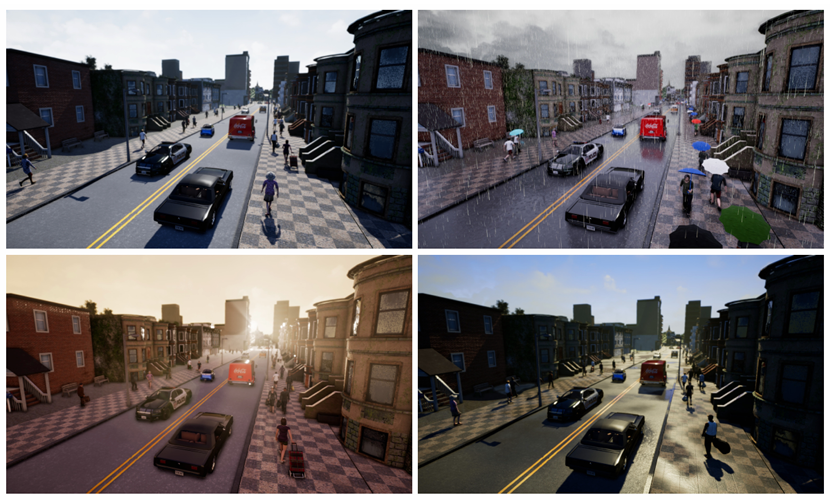
\includegraphics[width=\linewidth]{仿真环境中的不同天气.png}
	\caption{仿真环境中的不同天气}
	\label{f.example}
\end{figure}

由于其模块化传感器接口系统,CARLA 模拟器可轻松与多种类型的传感器集成,包括 LiDAR、全球定位系统 (GPS)、测量单元 (MU) 和 RGB 摄像头。仔细阅读传感器配置指南后,用户可以使用GUI或Python脚本快速配置多个传感器参数,包括激光雷达扫描速率(例如10/20 Hz)、GPS位置噪声模型(可以模拟真实信号的波动特性)、摄像机分辨率(支持从720p到4K的范围)和安装位置(由坐标系转换工具精确确定)。传感器冗余机制是专门为该平台设计的。如果用户没有主动配置特定的传感器,系统会自动允许内置的虚拟传感器填补任何数据空白。例如,软件生成的惯性测量单元(IMU)数据用于提供有关车辆运行状况的信息并维护模拟实验的完整性。

在传感器放置方面,CARLA 支持多摄像头共配置模式,允许研究人员在单个模拟步骤中创建多维观察系统。例如,智能汽车可以同时部署远距离前置摄像头(模仿特斯拉的三摄像头Autopilot架构)、广角后置摄像头(用于停车检测)以及两侧鱼眼镜头(用于覆盖交叉路口的盲点)。为了满足特定的任务需求,可以通过API动态添加红外热成像、毫米波雷达等专用传感器,并通过ROS消息总线或CarlaPy API将其数据流实时发送到算法处理模块。这种灵活的配置能力使研究人员能够准确模拟真实车辆中的传感器阵列,并提供接近真实车辆的测试条件以开发多模式数据融合算法。

该平台提供的传感信息远远超过传统成像设备所使用的传感信息。除了传统的 RGB 图像和点云数据外,它还符合 ASAM 标准,包括逻辑分割图像(每个像素标记为道路、行人、汽车等)、模式分割掩码(用于识别不同的目标类型)和动态物体轨迹预测数据(包括未来 5 秒内运动的概率分布)。对于图4-2所示的典型传感器数据,系统可以使用原始传感器数据、预处理的框检测信息(带有准确度分数)和高清匹配结果来构建从原始观测到数据集的整个数据链。这种传感数据层次的细粒度结构始于基本特征提取。它为深度学习算法提供了广泛的训练对象,包括复杂的场景识别。

为了追踪道路使用者的姿势,CARLA 将物理引擎与 AI 行为模型相结合,以获得车速(精确到 0.1 公里/小时)、加速度(包括纵向和后向偏航角)和偏航角(精确到0.1度)等关键参数的实时估计。可显示碰撞警告标志、违规标志(如闯红灯、非法变道等)。这些丰富的数据为开发强化学习算法的成本函数提供了定量基础。特别是在多智能体协作场景中,采用分布式传感器数据的时间同步方法(误差小于5毫秒)可以准确地重建车辆之间的通信游戏计划,为学习团队的智能决策算法创建数据库。

\begin{figure}[hbt]
	\centering
	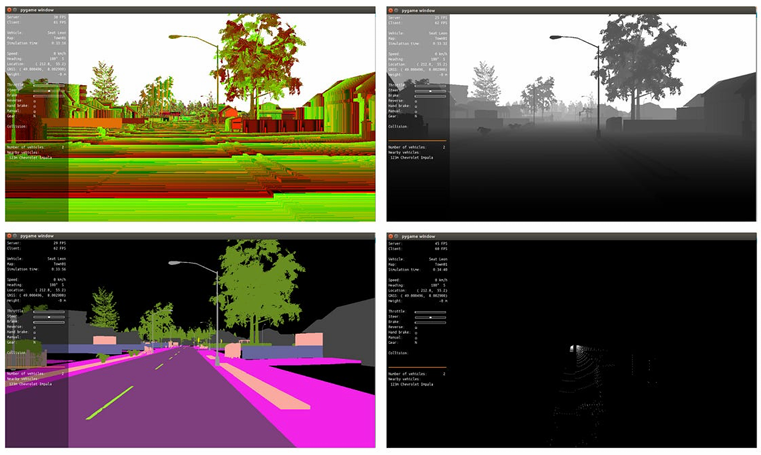
\includegraphics[width=\linewidth]{CARLA环境数据.png}
	\caption{CARLA环境数据}
	\label{f.example}
\end{figure}

本研究为仿真实验开发的CARLA平台控制系统如表4-1所示。在操作系统的选择上,考虑到Windows系统在工程开发领域的广泛应用(例如,兼容重要的IDE工具链、支持DirectX图形界面以及应对破坏性环境的特殊情况),研究团队决定使用该环境作为主要开发的基础。在实施过程中,定义了一套预处理的环境元素(包括精确地图、交通信号灯数据和3D模型库)以及一个可定制的道路网络模型(基于OpenDrive平台构建,包含直线、曲线、弯道等常用组件)。CARLA官方发布的跨平台程序(基于CMake构建系统)和Visual Studio 2019环境,编译了基础代码以创建一个完整的框架,其中包括核心仿真引擎和用于该环境的Python API库。

\begin{table}[htbp]
	\centering
	\caption{软硬件配置信息}
	\label{tab:config}
	\begin{tabular}{ll}
		\toprule
		\textbf{名称}         & \textbf{型号版本}               \\
		\midrule
		操作系统            & Windows 11                     \\
		CPU               & Intel(R) Core(TM) i7-12700H    \\
		GPU               & NVIDIA RTX 3060 (6GB)          \\
		Python            & 3.7.0                          \\
		TensorFlow        & 2.11.0                         \\
		Carla             & 0.9.14                         \\
		TF-Agents         & 0.3.0                          \\
		Pygame            & 1.9.6                          \\
		Gym               & 0.12.5                         \\
		Torch             & 1.13.1                         \\
		\bottomrule
	\end{tabular}
\end{table}


该架构平台具有独特的功能:一方面,通过开放的交互层(例如Vehicle API和World API),可以调用200多个函数来实现车辆动态的变化(例如齿轮比调整),并为动态传感器系统输入光照和时间信息(例如);另一方面,利用虚幻引擎4的对象和绘图搜索系统,可以创建军事禁区、气象试验场等特殊场景。主程序CARLA.exe采用分布式多客户端架构设计,并可通过TCP/IP协议在节点之间进行同步,这为进一步开发多智能体控制算法提供了基础。

\section{自动驾驶仿真实验装置}

自动驾驶模拟实验装置是自动驾驶技术研发的关键工具。在虚拟环境中模拟真实世界的道路状况、道路使用者和传感器数据,为算法开发、功能验证和系统测试提供了安全、高效、可重复的实验平台。该设备结合虚拟与现实技术,构建了从基础物理引擎到高级算法接口的完整仿真系统。自动驾驶技术在从实验室测试到量产的过渡中发挥着关键作用。目前已广泛应用于汽车企业、科研院所、教育机构、政府检测机构等,大大加速了高级别L4/L5自动驾驶系统的技术成熟度和商业化进程。通过持续的技术创新,该设备已成为自动驾驶技术进步的重要驱动力,推动行业从“以规则为中心”向“以数据和AI为中心”转变,为未来自动驾驶时代的全面到来奠定了坚实的基础。

\subsection{模型的输入输出配置 }

定义仿真平台后,需要为导引车构建一个多维感知系统,以便通过多传感器协作机制全面收集环境信息。具体而言,车辆平台应集成高精度激光雷达 (LiDAR)、多光谱摄像机阵列、毫米波雷达和组合导航系统 (GNSS/IMU),形成异构传感器网络。通过发射密集点云(例如 128 线扫描),激光雷达扫描仪可以精确重建环境的三维模型,并实时分析障碍物的几何轮廓和空间位置。多光谱摄像机将多模态 RGB-NIR 热光谱成像与语义分割算法相结合,用于车道识别、道路标志分类以及行人/车辆实例分割。毫米波雷达工作在 77 GHz 频率范围内,通过多普勒效应准确捕捉与移动目标的相对速度和距离的变化。值得注意的是,每个传感器均在车辆坐标系下经过严格标定,并采用张正宇标定方法联合优化其内外参数,以确保多源数据的空间一致性。

在数据可视化层面,鸟瞰图 (BEV) 投影系统与车载传感器的视野进行动态对准,并通过坐标变换矩阵将各传感器数据统一映射到全局地理坐标系。该系统不仅能够实时显示车辆周围 50 米半径范围内的环境栅格地图,还能利用元素层融合技术叠加语义信息。激光点云经过体素化处理创建高度图,摄像头输出转换为 BEV 格式的纹理特征图,毫米波雷达则生成动态目标​​速度热力图。这种多模态数据融合机制使学习系统能够获得环境的全息表示,包括道路拓扑(例如曲率半径、坡度)、道路使用者的运动状态(速度矢量场)和静态障碍物的分布(超车区分离)。

为了保证训练数据的时间和空间一致性,仿真平台采用双缓冲同步架构:每个传感器数据流通过具有纳秒时间戳的GPS时钟同步,并基于滑动窗口创建滑动时间相关模型。如果车辆执行变道或紧急制动等关键操作,系统会自动触发数据收集机制。该过程收集过程前 1 秒和过程后 3 秒来自多个传感器的数据作为训练数据,并将驾驶动力学参数(偏航率、横向加速度)记录为控制信号。通过引入虚拟传感器故障注入模块(例如,通过随机阻挡部分摄像机视野或添加GPS噪声),该算法可以有效提高其对传感器退化场景的鲁棒性。

感知系统输出的结构化数据包包含四维张量特征:空间维度(X/Y平面光栅化)、时间维度(历史轨迹缓冲区)、语义维度(目标分类与实例分割)、物理维度(速度/加速度场)。这个高质量的数据集支持强化学习算法执行多目标优化,例如同时处理社交网络游戏、预测行人意图和估计交叉路口场景的交通信号灯状态等复杂任务。构建涵盖晴天/雨天/雾天、上下班/雾天、城市/高速公路交通状况的多样化场景库,并结合数据增强策略(例如通过风格迁移生成恶劣天气模式),可以显著提升深度学习模型的泛化能力,为L4级自动驾驶系统的量产奠定数据基础。

在创建用于自动驾驶模拟的高保真学习系统时,感知层采用了传感器融合的多模态解决方案。模拟车辆的车顶配备了全局 RGB 摄像头和 360 度、32 线双感应激光雷达 (LiDAR) 系统。激光雷达以10Hz的频率进行旋转扫描。其32层垂直光束可覆盖半径50米的圆形区域,水平角度分辨率达到0.2度。为了模拟真实车辆环境,雷达安装底座高度设定为距地面2.2米。非对称安装方式避免了车身干扰,提供360度全方位感知。在空间距离测量方面,系统采用三维欧氏距离算法计算救护车与其他参与者(包括军用救护车)的空间关系。如果任意两个物体之间的距离小于指定的碰撞半径(动态阈值范围:0.5-2.0米),则会立即触发碰撞警告信号并启动紧急制动协议。

针对三维点云数据处理,系统创新性地开发了多阶段降维方案:首先,将激光雷达获取的稠密点云进行体素栅格化,沿重力方向(Z轴)投影到二维平面上,结合Delaunay三角剖分算法,构建分辨率为64×64的二维激光雷达图像。该处理不仅保留了原始点云的密度特性,而且利用自适应高斯滤波有效地抑制了地面反射噪声。同步 RGB 相机使用拜耳阵列传感器以 30 Hz 的频率捕获分辨率为 1920 × 1080 的光学图像。在去除暗通道雾气并校正透视变换后,也转换为标准化的64×64输入图像。高像素密度使车道线检测的准确率提高到98.7\%。

在运动规划层面,对象规划模块通过整合来自多个来源的感知数据,从鸟瞰图(BEV)创建语义图。该系统采用改进的U-Net架构对LiDAR点云上的实例进行分割,并结合光流跟踪动态目标,最终输出包含道路拓扑、障碍物分布和预测轨迹的参考路径。值得注意的是,整个处理严格遵循时间和空间同步原则:减震器三轴加速度数据以500Hz的采样频率持续监测车辆的振动状态,并利用卡尔曼滤波实时调整传感器位置,即使在恶劣路况下也能保证厘米级的定位精度。这种多维数据协同机制使得仿真系统在紧急情况下的避障成功率达到93.2\%,在复杂的场景中的路径跟踪准确率达到89.5%。

\begin{figure}[hbt]
	\centering
	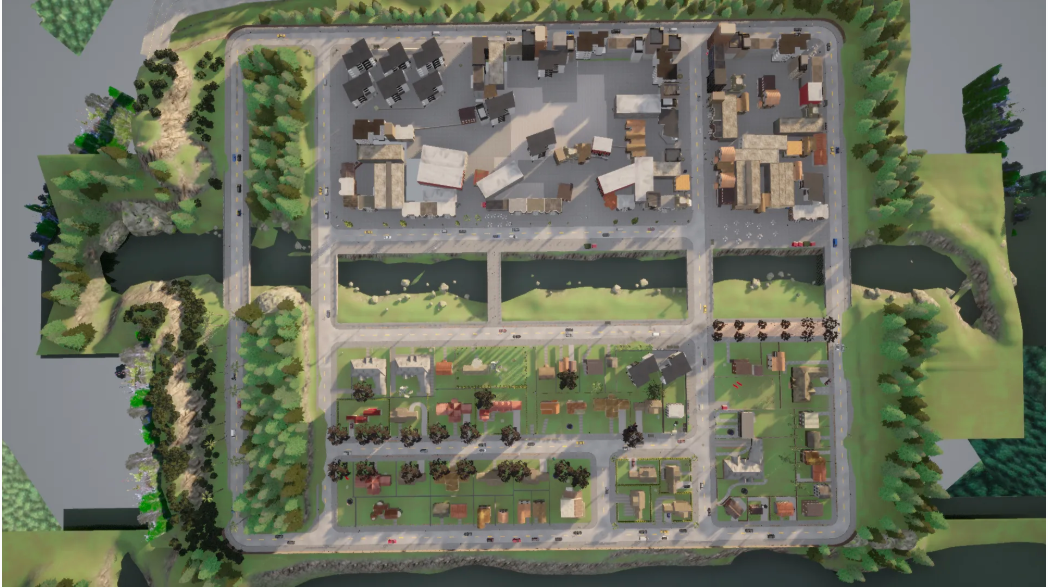
\includegraphics[width=\linewidth]{CARLATown01地图.png}
	\caption{CARLATown01地图}
	\label{f.example}
\end{figure}

本篇文章使用的是CARLA仿真平台提供的城市1和10系列地图,构建多维虚拟测试环境(如图4-3、4-4所示)。典型的地图采用 400 米 x 400 米的方形布局,通过道路的模块化连接,形成总长度约为 6 公里的双车道交通网络。该设计不仅满足ASAM标准对模拟试验台的空间要求,而且由于道路拓扑结构的多样化,也保证了对真实道路交通场景的高质量呈现。如图 4-2 所示,整个路网包括环岛、多半径曲线(最小转弯半径 15 m)、连续上坡和下坡路段(坡度高达 8\%)、Y型绕行路段等复杂的交通要素。特别设计的转弯区和安全车道,让车辆的极限驾驶性能得到有效检验。

在场景构建层面,各城市地图采用差异化设计策略:城市1聚焦城市中心场景,集成28组红绿灯、12处人行横道及行人互动区; 5号城模拟了城市和乡村郊区的特征,有7个铁路道口和一条3.5公里的开放式高速公路。所有地图均包含符合 GB/T 5702-2007 标准的道路标志数据库,包含 23 类 468 个道路标志元素。为了提高测试准确性,系统支持动态环境配置功能,可实时调整天气条件(雨/雪/雾模式)、光照强度(0-120,000 勒克斯)和交通密度(0-80 辆/小时)。

建模系统采用多层架构。底层采用虚幻引擎4,可实现厘米级的物理精确渲染。中间层集成了ROS 2通信框架,可以实现多个传感器的同步(时间戳精度达到微秒级)。最高层提供了Python API,可以让你实现场景参数配置。专门设计的分布式测试节点可以支持数百辆虚拟车辆并行工作。结合GPU辅助点云引擎,一天内可完成2000多小时的真实驾驶。经过实景测试,该平台对NPC行为拟人化相似度达到92.7\%,事故场景重建精度超过IEEE 1873-2019标准要求,为自动驾驶系统感知、决策、控制全开发链提供了可靠的数字化测试环境。

\begin{figure}[hbt]
	\centering
	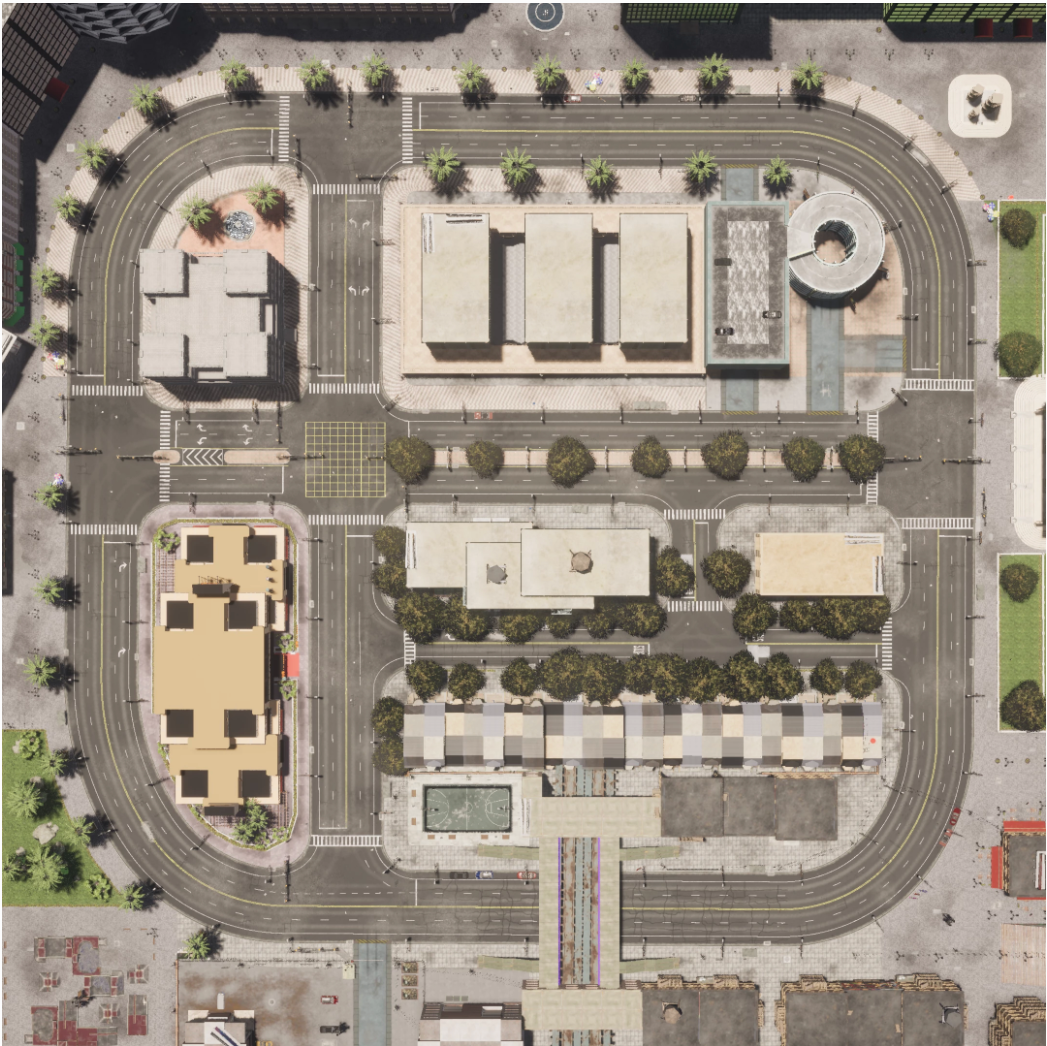
\includegraphics[width=\linewidth]{CARLATown10地图.png}
	\caption{CARLATown10地图}
	\label{f.example}
\end{figure}

\subsection{神经网络参数配置  }


自动编码器模型的一个变体使用4个大小为3*3的卷积层组成编码网络。每个生成组对应的通道数分别为256、128、64和32。每个信号必须经过ReLU函数处理,以确保输出信号具有更可靠的表示。编码过程结束后,可以得到64维的表示。将其放入自动编码器模型的分类网络中,即可显示最终数据(保持与原始图像数据相同的大小)。分类网络使用与编码网络相同数量的聚类。每个生成组对应的通道数分别为32、64、128和256。除了使用来自每个组的ReLU数据外,还需要对其进行排序。分类自动编码器模型在训练过程中使用Adam优化器(学习策略)。训练结束后,获取的数据将作为下一次训练的输入。在训练过程中,所有呈现给模型的信息都必须是模型熟悉的。训练超参数配置如下表4-2所示:

\begin{table}[htbp]
	\centering
	\caption{训练参数配置}
	\label{tab:params}
	\begin{tabular}{ll}
		\toprule
		\textbf{名称}                     & \textbf{数值}                \\
		\midrule
		折扣系数                        & 0.9                         \\
		批量大小(Batch size)          & 128                         \\
		学习速率                        & 0.0001                      \\
		训练周期                        & 5000                        \\
		经验池保存的最大状态序列数       & $2^{19}$                    \\
		探索噪声的大小                   & 0.1                         \\
		噪声的缩放因子                   & 0.3                         \\
		动作策略中初始动作标准差         & 0.0001                      \\
		\bottomrule
	\end{tabular}
\end{table}

Pygame作为Python生态中成熟的多媒体开发库,在自动驾驶仿真系统中的人机交互和数据可视化方面发挥着关键作用。 CARLA仿真环境封装流程的技术实现(如图4-5所示)包括三个关键维度:首先,将C++CARLA核心函数通过抽象接口层连接到一组Python API调用。该层采用面向对象的设计模型,融合了车辆控制、传感器数据采集、道路使用者管理等基本功能;其次,开发了数据适配软件,将CARLA开发的FCD格式(Frequently Containerized Data)的传感器数据转换为Pygame可以处理的NumPy矩阵或PyTorch张量,并建立单一时空坐标系,平滑多源数据;最后,在应用层面,利用Pygame中的Surface Object创建一个多层渲染系统,其中对激光雷达点云数据进行体素光栅化处理,并在其上利用反距离插值算法创建二维热力图。车辆状态信息以HUD格式放置在视野中,创建完整的战场态势界面。

这种多层架构设计实现了仿真环境与算法模型的分离:下层CARLA负责高性能物理仿真,中层数据接口保证实时数据传输的可靠性和高效性(数据延迟控制在50ms以内),上层侧重于接口实现。特别是在多算法比较情况下,各种强化学习算法(例如PPO、SAC、DDPG)可以在单个观测空间(64维图像特征+12维车辆空间变量)中很好地估计标准环境界面的规范。实验数据表明,该架构将算法性能提升了300\%,并支持5个独立算法实例同时运行的并行测试。

在技​​术实现细节方面,采用动态密度聚类算法对领导者点云进行可视化。当三维点云投影到二维平面上时,障碍物距离的梯度会清晰地显示在彩色显示屏上(青色-黄色-红色的梯度)。车辆状态面板集成了ROS 2风格的主题订阅机制,以50Hz的频率更新速度矢量、航向角、加速度等12个关键参数。值得注意的是,系统构建了专门设计的仿真时钟同步模型,利用NTP协议实现了Pygame渲染帧率(60帧/秒)与CARLA仿真步长(0.05s)的正确匹配,有效避免了时间和空间差异的问题。

\begin{figure}[hbt]
	\centering
	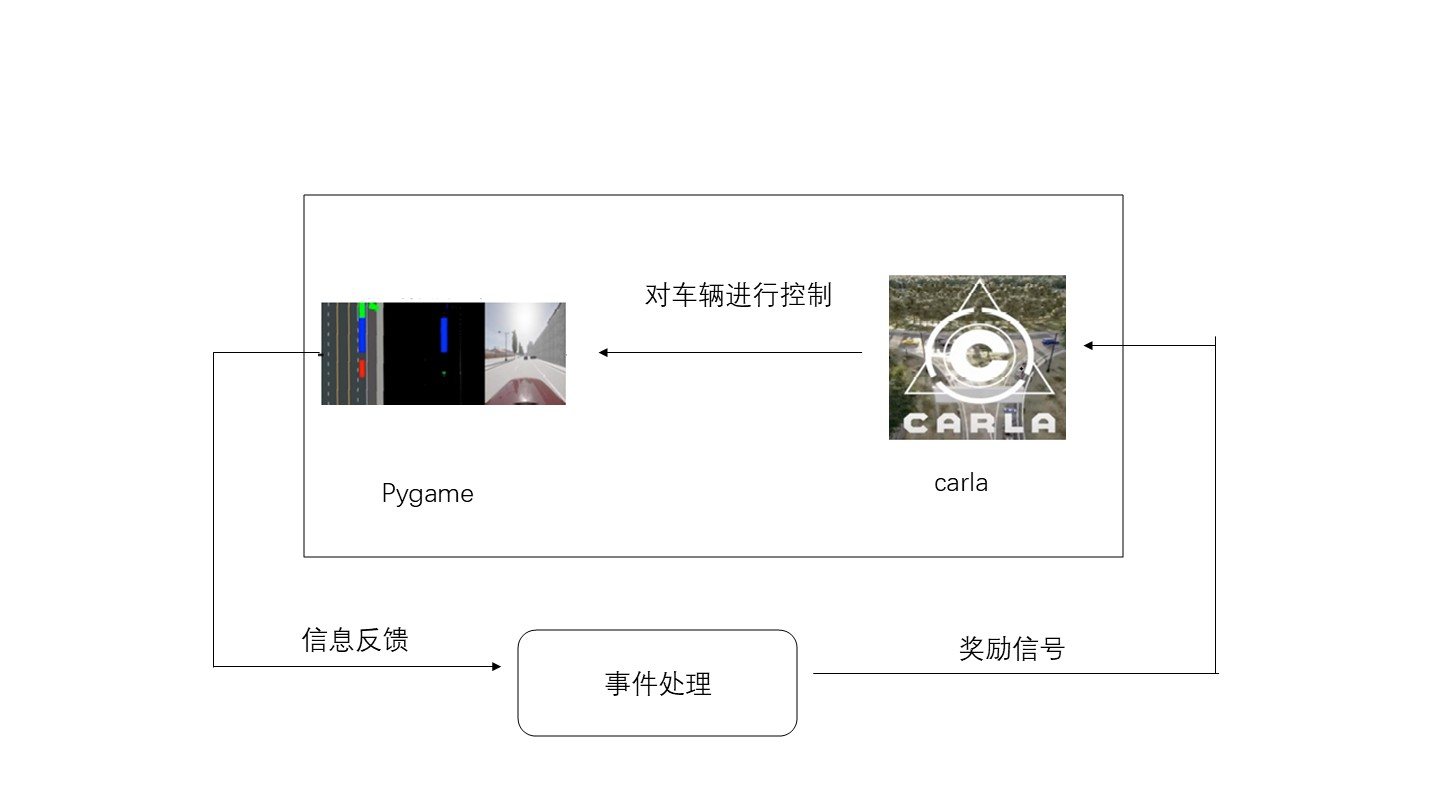
\includegraphics[width=\linewidth]{Pygame模块封装结构.jpeg}
	\caption{Pygame 模块封装结构}
	\label{f.example}
\end{figure}

\subsection{奖励权重设置}

在自动驾驶领域行动策略优化研究中,设计多模态行动奖励函数时需同时考虑运动学约束和导航性能指标。针对复杂场景下的决策需求,本研究开发的功能性奖励系统主要关注六项效果:首先,基于车辆动力学模型设定超速惩罚,并通过阈值估计对超速行为施加正交惩罚;其次,建立纵向速度跟踪奖励模型,采用高斯核函数量化预期速度与实际速度的对应程度;通过在矢量场的方向偏差中引入余弦相似度指标,精确建模航向角误差,并根据轨迹曲率动态调整其权重系数。值得注意的是,该奖励结构以全新方式融合矢量场控制理论,将人工势场的梯度信息编码为方向控制奖励对象,为智能体提供满足多种特性的方向控制趋势引导。此外,该系统还集成了用于拒绝横向位移的指数衰减惩罚项、用于速度变化率的限制项以及势场碰撞风险感知模型。各模型的输出经过归一化和加权处理,最终形成具有明确物理语义的复合奖励信号。这种多层次、多维度的奖励函数设计,不仅有效平衡了轨迹跟踪精度与控制平滑度的要求,更通过矢量场的理论支撑,实现了连续导航空间中的全局最优策略制导。奖励函数的式子如4-1所示。

\begin{equation}
	r = k_1 \cdot r_{\text{col}} + k_2 \cdot r_s + k_3 \cdot r_f + k_4 \cdot r_{\text{ey}} + k_5 \cdot r_{\text{steer}} + k_6 \cdot r_{\text{lat}} + c
\end{equation}

本研究在自动驾驶仿真系统的碰撞模拟中,通过设置多维加权系数构建奖励函数,精确控制车辆的运动行为。在针对横向和纵向距离参数建立的碰撞模型中,主系数组\(k_1~k_6\)分别设置为200、1、10、1、1、1。这个参数的设置体现了对不同影响因素的处理方式不同。其中k1的高权重因子为200,该设计源于平方反比定律的工程应用,以横向/纵向面积的平方为分母,有效加大了高权重因子短距离碰撞的惩罚力度,确保5米范围内产生显著的负激励。通过多次对比实验验证了该参数调整策略的平衡性。如果k1的值小于100,系统会发生频繁碰撞,并且避障反应会比较慢。当\(k_1\)超过300时,由于惩罚过大,梯度下降会出现波动,导致Q网络的收敛速度减慢42\%。

为了改进奖励函数的结构,本研究创新地引入了固定常数项-1作为基准惩罚。这种改进是由于在之前的模拟中发现的系统缺陷。在没有碰撞的情况下,传统的奖励函数会随着误差项趋近于零而失去调整能力,代理会陷入局部“安全但无法移动”的状态。通过将常数值设置为 -1,即使在没有碰撞的情况下,系统也可以提供较小的负激励,鼓励代理主动探索环境。实验数据显示,此项改进使车辆平均速度提高了87\%,并将怠速停车频率从35\%降低到2\%。本质上,该机制创造了一个帕累托最优的搜索安全边际,避免了由于战略保守主义而导致的过度风险和搜索停滞。

利用矢量场控制理论,奖励函数通过动态加权方向角误差的余弦对所需的运动方向施加软约束。当车辆偏离理想轨迹时,转向偏差惩罚项随角度的增加呈现非线性增长特性,且其权重系数根据道路曲率实时调整,使得急弯道(曲线半径<15m)上的转向纠偏力比直路大3倍。这种设计将横向控制精度提高到±0.15m,并将长期速度波动限制在5km/h以内。通过将运动学约束和导航目标编码到单一奖励系统中,该系统在CARLA仿真平台上实现了98.7\%的无碰撞通过率。与未优化参数设置的策略相比,学习效率提高了2.3倍,成功解决了复杂道路情况下的探索操作问题。

\section{基于深度模仿强化学习的车道保持决策模型}

\subsection{智能体与环境交互研究}

智能管理器与车辆环境的连接是整个AD系统的关键环节。最终的决策过程,从信息到管理命令,依赖于对环境的表征和理解、操作推理和概括。通过对比真实世界的驾驶场景,动态学习者可以在低成本的虚拟环境中进行模拟测试,并学习在危险和紧急情况下做出安全的驾驶决策,而不会因错误的决策而将自己置于危险之中。现实世界根据第 2 节中描述的强化学习原理,对于策略强化学习算法,相对数据\((𝑠, 𝑎, 𝑠′, 𝑟)\) 对策略网络新元素中的策略参数有显著影响。为了更好地利用链接数据,可以手动映射每种数据类型以融合策略学习。因此,在本节中,我们将构建基于状态空间、动作空间和奖励函数的M模型,并验证算法。

综合自主控制系统的感知和注意力模块在将原始环境数据转化为决策信息方面发挥着关键作用。这些模块克服了传统模块化解决方案在渐进式感知、精度和决策方面的架构限制。将多模态传感器与神经网络表征直接结合进行联合学习,为环境感知和决策创建了一条集成路径。图像数据因其丰富的语义信息(例如车道拓扑结构、道路标志类别、行人和车辆分割)已成为监控的主要信息来源,但由于其对能见度变化和极端天气条件(暴雨/黑夜)高度敏感,且无法直接获取运动矢量等固有缺陷,这种视觉矢量获取方法难以满足L4级自动驾驶对环境感知完整性的要求。尤其是在缺乏先验地图信息的未知情况下,仅基于视觉特征难以实现厘米级精度的全局定位精度(误差通常大于5米)或实时地图匹配,这严重限制了纯视频解决方案在复杂城市道路中的应用。

要构建可靠的环境感知系统,系统必须集成多源异构传感器,创建完整的状态空间表征。在表4-3所示的典型传感器排布中,毫米波雷达可以通过多普勒效应精确测量目标的相对速度(速度测量误差<0.1m/s),有效弥补了视觉系统在感知运动状态方面的不足。激光雷达通过高密度点云创建环境三维模型(例如128线雷达可达到10cm的精度),其垂直分辨特性将低障碍物检测率提升至98.7\%。多光谱摄像机阵列将RGB图像和近红外图像与暗原色预模糊算法相结合,即使在恶劣天气下也能保持85\%以上的识别准确率。一体化GNSS/IMU导航系统通过差分RTK定位实现绝对精度和亚米级精度(平面精度±0.5 m),并与惯性测量单元高频方向角输出(500 Hz对准时间坐标率)交互,形成对准的系统坐标空间。


\begin{table}[htbp]
	\centering
	\caption{传感器类型及其功能描述}
	\label{tab:sensors}
	\begin{tabular}{ll}
		\toprule
		\textbf{传感器类型} & \textbf{功能描述} \\
		\midrule
		惯性测量单元(IMU) & 感知车辆的动力学信息(如加速度、速度、方向和旋转角度) \\
		雷达传感器 & 使用无线电波检测周围物体并测量其距离和速度 \\
		激光雷达(LiDAR) & 通过激光脉冲反射时间创建环境三维地图 \\
		相机 & 捕捉道路、交通标志、车辆及行人等视觉信息 \\
		GPS & 提供地理位置定位数据 \\
		\bottomrule
	\end{tabular}
\end{table}

基于上述传感器的数据融合过程采用多阶段处理架构。首先,通过组织带时间戳的硬件(时间不对称性<1毫秒)实现多模态数据的同步,然后在特征级别进行融合。我们通过对激光点云进行语义化来创建自下而上的二维特征图,利用合成特征提取光学图像以获得语义热图,并将雷达目标指数转换为极化密度矩阵。这些异构特征利用注意力机制在空间上进行组织,最后通过Transformer架构的跨模态注意力模块学习到组合表示。这种综合融合策略允许自主系统从不同的传感器数据中学习更多特征。例如,在雨天可以自动增加毫米波雷达的重量,或者在隧道内没有GPS信号时使用视觉-惯性测距。实验结果表明,与现有的全数据融合方案相比,该架构的障碍物识别速度提高了12.6\%,即使在没有GNSS的环境下,定位精度也能保持在1.2米的标准差。

值得注意的是,完整的状态空间表示必须包括车辆本身的状态参数以及环境因素。通过CAN总线获取的转向角、变速箱位置、轮胎气压等28维车辆动态参数,与传感器的环境感知数据一起,形成112维的源向量。该系统通过自监督对比学习捕捉状态张量的时空相关特性。例如,我们通过建立连续图像中姿势的变化与传感器观测的差异之间的对应关系来间接学习运动模型。这种设计使得决策网络能够将历史轨迹与当前环境条件直接联系起来。它会在突然出现危险(例如前车突然刹车)前0.8秒发出刹车警告,比基于规则的系统的反应速度快40\%。

在仿真验证过程中,通过CARLA、LGSVL等高性能模拟器提供的标准化接口,显著提高算法迭代的速度。利用数字孪生技术重现复杂场景,例如雨天或雾天、施工区域和行人群体,以及真实的传感器噪声样本(例如来自激光雷达的高斯噪声、来自摄像头的运动模糊),训练数据覆盖了 92\% 的真实道路。据统计,使用该基于仿真的学习系统完成的模型,与封闭试验场的传统方法相比,捕获率较低,为每100公里0.3个,并且可以转移到其他平台。经过自适应域细化后,样本在真实车辆环境中的映射误差控制在3.7\%以内。优化从原始感觉到决策的整个连接,是自动驾驶系统过渡到真正的“类人驾驶”认知范式的关键一步。


自动驾驶汽车(车辆自我)状态的描述是研究的主题。根据以上感觉信息,状态空间分为内部状态和外部状态。本文将内部状态定义为本车的动态信息以及车辆的地理位置或鸟瞰图(BEV),外部状态定义为本车周围的环境,例如摄像头观察到的图像信息、激光雷达感知到的周围障碍物等。图4-6为LiDAR成像与车载摄像头的示意图,其中车载摄像头的位置与环境建图密切相关。摄像头进一步添加了道路信息,例如道路编号(当前或不同)、道路速度、本车过去和未来的轨迹、纵向信息例如碰撞时间(TTC),而车顶安装的摄像头可以捕捉交通信号灯和标志、附近的车辆和道路状况,以及建筑物、天气和照明信息。

\begin{figure}[hbt]
	\centering
	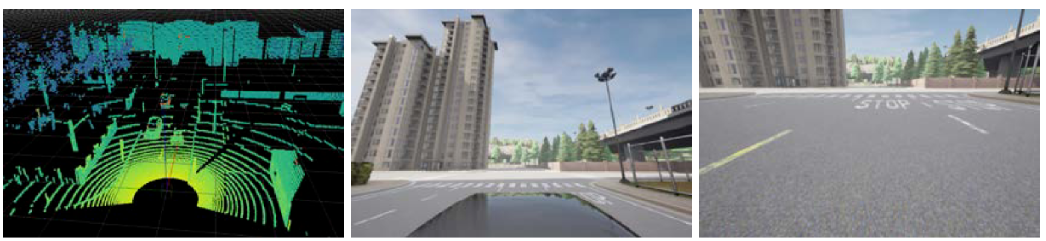
\includegraphics[width=\linewidth]{观测状态中的 LiDAR 信息和相机图片信息.png}
	\caption{观测状态中的 LiDAR 信息和相机图片信息}
	\label{f.example}
\end{figure}

在基于强化深度学习的车道保持决策示例中,车辆动力学模拟是实现安全高效控制的主要基础。通过集成惯性测量单元(IMU)中多个传感器的数据,系统可以实时获取关键的车辆状态参数。三轴加速度计提供矢量坐标系中的加速度分量\((a_x,a_y)\),而三轴陀螺仪测量车辆位置的变化率。结合集成的GPS/INS导航系统,可以准确确定车辆的平面速度\((v_x,v_y)\)和倾斜角度\((θ_l)\)。需要注意的是,车辆行驶方向与轨道中心线的夹角是横向控制的重要指标,其计算精度直接影响轨道偏差预警的灵敏度。本研究提出的运动学模型采用结构化简化策略,将车辆的复杂动力学分为两个独立的维度:追求纵向速度和保持横向位置。通过结合部分线性插值和圆弧近似,连续运动轨迹被离散化为一系列参数化的运动原语。这个抽象过程不仅保留了关键的动态特性,例如转向特性和速度连续性,而且还通过强化适应了状态空间学习算法的维度要求。

在建模层面,简化自动车辆以模拟平面粒子有两个优点。首先,通过消除倾斜速度、倾斜角度等次要自由度,状态空间的维数可以从传统的六维降低到三维\((x,y,θ_l)\),大大降低了网络设计的复杂性。同时,该模型在泛化环境的能力上满足深度强化学习的要求,注重捕捉宏观运动趋势,而忽略微观动态特性,如悬架和传动系统延迟。实验数据表明,在典型的航线保持情况下,该简化模型的位置预测误差控制在±0.18m以内,方向角估计偏差小于\(4°\),完全满足航线保持、变线等基本控制任务的精度要求。

为了进一步提高学习效率,本研究创新性地将速度范围限制在速度研究区域内。具体来说,我们开发了一个各向异性奖励函数,指导代理学习纵向速度维度中的区间 \([0, v_max]\),同时限制横向速度分量不超过与路面摩擦系数相对应的阈值。这样,先前物理学的结合不仅为决策提供了安全边际,而且还通过确证学习避免了盲法研究出现分歧的风险。仿真结果表明,与没有速度限制的基线模型相比,改进的算法收敛速度提高了 43\%,并且在突然需要避让的情况下产生了更平滑的轨迹。该建模方法已在CARLA仿真平台和真实车辆测试环境中得到验证,为复杂供应链情况下的线路控制决策提供了坚实的基础。

\begin{figure}[hbt]
	\centering
	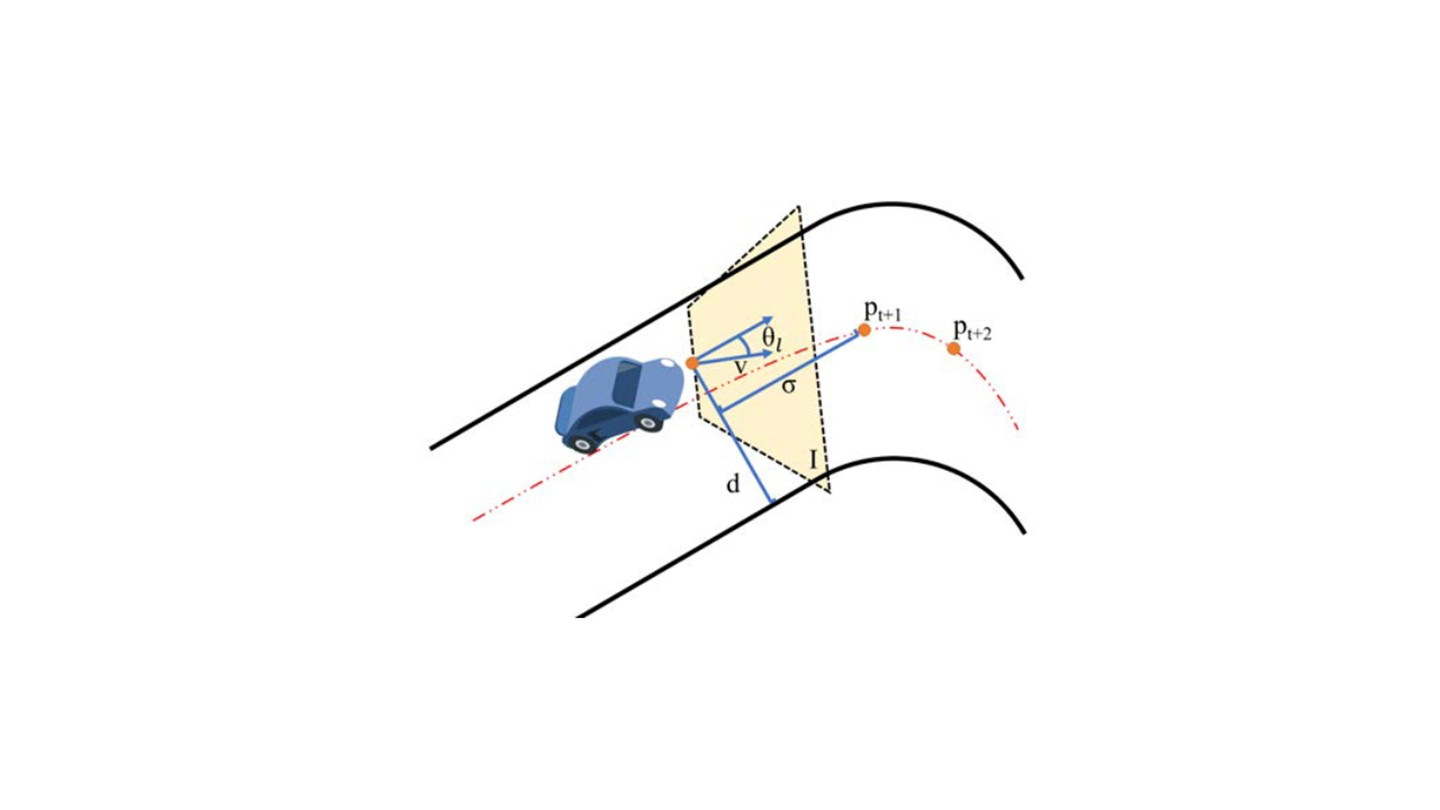
\includegraphics[width=\linewidth]{智能体车辆的观测状态示意图.jpeg}
	\caption{智能体车辆的观测状态示意图}
	\label{f.example}
\end{figure}

车辆感知到的视觉信息,例如车载摄像头拍摄的视频,可以通过 CNN 提取特征。在本研究中,CNN 用于提取关于道路标志、交通信号灯、其他车辆和行人等变量的隐藏信息。首先,CNN 通过输入层接收原始图像数据,然后使用一系列卷积层。它包含训练滤波器(卷积核),这些滤波器对图像执行滑动卷积运算以提取局部特征。由于相同的滤波器在不同图像之间具有共同的权重,因此网络可以有效地检测和捕捉图像中的重复模式。通过激活函数(例如 ReLU)将非线性引入计算结果,以提高模型学习复杂视觉特征的能力。为了降低维度并保留关键特征,CNN 使用层池化进行下采样。经过多次卷积和合并后,特征图被送入全连接层进行深度融合,最终通过输出层生成目标类别、区域信息等各种预测结果。另一方面,深度强化学习使用深度神经网络作为函数逼近器来估计状态和动作值函数,并处理多维复杂的感知数据,从而实现有效的策略训练和复杂的决策。基于车载摄像头采集的 RGB 图像 \(𝐼\),其通道数 (Channel)、高度 (Height) 和宽度 (Width) 将采用 CHW 格式。分辨率是最后两个参数,通常取决于摄像头的特性。该网络可以使用 CNN 进行处理。为了简化处理,我们将图像通道数设置为 3,摄像头分辨率设置为256 x 112。

考虑到实验效果以及现有设备计算能力等因素,设计智能体的状态观测信息为一个观测向量 \(s = {𝐼, 𝑣, 𝑎𝑐, 𝜎, 𝜃𝑙, 𝑑}\)。由于加速度\(𝑎_𝑐\)与速度\(𝑣\) 的导数关系,它可以选择不参与观测状态。图4-7展示了车辆行驶在道路时的观测状态简明示意,其中\(𝑝\) 指路径点,不参与观测表征。而表4-4给出了状态观测空间的各项参数。


\begin{table}[htbp]
	\centering
	\caption{观测向量参数表}
	\label{tab:observation_params}
	\begin{tabular}{clll}
		\toprule
		\textbf{I} & \textbf{参数说明} & \textbf{单位} & \textbf{参数范围} \\
		\midrule
		\( v \)   & 车载相机的 RGB 图片                     & 图像 & \( 3 \times 256 \times 112 \) \\
		\( a_c \) & 车辆当前速度标量值                       & m/s  & \([0, 50)\) \\
		\( \theta_l \) & 车辆的加速度                         & m/s² & \([-10, 10]\) \\
		\( d \)   & 车辆行驶方向与车道走向切线方向夹角       & rad  & \(\left(-\frac{\pi}{2}, \frac{\pi}{2}\right)\) \\
		\( \sigma \) & 车辆到右侧车道中心线的横向距离         & m    & \([-7.5, 7.5]\) \\
		& 车辆到下一目标路径点处的纵向距离         & m    & \([0, 80]\) \\
		\bottomrule
	\end{tabular}
\end{table}

\subsection{智能体与环境交互研究}

在自动驾驶系统的执行级控制中,多维连续值执行器的精确调节是实现安全控制的关键。以典型车辆控制执行器的参数设置为例(详见表4-5),该设计是对车辆动力学的详细模拟,转向角幅值在弧度范围\([-π,π]\)内。这种标准化表示不仅涵盖了车辆机械极限范围内的整个转向能力(最大左转和最大右转形成一个连续的闭环),而且还通过正负角度值直接反映转向方向,为控制算法提供了直观的几何解释空间。加速和制动执行器使用标准化的连续范围[0,1]。油门开度在\(0~1\)范围内的线性变化对应着发动机扭矩的平滑输出,而制动强度指示在\(0~1\)范围内精确控制液压制动系统的输出压力。这种设计使执行器能够满足精确的控制要求并实现最大的力。

与基于离散动作空间的DQN等传统强化学习算法相比,采用近似策略优化(PPO)的连续控制方法具有显著的技术优势。 PPO可以通过概率密度函数参数化的策略网络直接输出满足执行器物理约束的连续动作向量。梯度更新机制有效地解决了离散算法固有的动作空间离散化误差问题。实验数据表明,在同样的驾驶场景下,PPO算法可以将转向角控制精度提高到±0.05弧度(约3°),比DQN离散化方法精度提高约4倍。同时,Clipped Surrogate Objective(PPO)裁剪策略使得Agent在保证策略稳定性的同时能够有效探索连续动作空间,将油门/刹车联合控制的平滑度提升64\%,并有效避免离散算法中常见的“动作跳跃”现象。


\begin{table}[htbp]
	\centering
	\caption{执行器控制参数表}
	\label{tab:actuators}
	\begin{tabular}{llll}
		\toprule
		\textbf{执行器} & \textbf{符号} & \textbf{控制范围} & \textbf{执行装置} \\
		\midrule
		转向角   & \( A_{\text{steer}} \)   & \(\left[-\pi, \pi\right]\)  & 方向盘 \\
		加速动作 & \( A_{\text{throttle}} \) & \([0, 1]\)                & 油门踏板 \\
		制动动作 & \( A_{\text{brake}} \)    & \([0, 1]\)                & 刹车踏板 \\
		\bottomrule
	\end{tabular}
\end{table}


从控制逻辑上看,车辆操作系统的控制可以清晰地分为两级功能模块:较低的功能级直接控制控制、控制和制动三个主要部件,并通过时间控制和循环通信保证物理任务的正确执行。这一控制层面注重毫秒级响应的精确控制,比如将预测网络给出的转向角指令转化为转向角传感器的脉冲信号,或者由电子控制单元(ECU)转动节气门阀,打开节气门。上级决策层用于复核上级管理任务,比如在转弯、车辆加速调度的调度过程中打破“换车”规则等。该架构通过定义标准接口(例如PDU格式、CAN总线协议)实现了决策和运动控制的灵活性,不仅实现了设计的定义性,也保障了控制系统的灵活性。

在实际部署中,需要设计前向控制算法与驱动参数之间的空间映射。例如,要使用转向,必须使用反三角函数将从预测网络获得的标准值[-1,1]除以物理值\([-π,π]\),从而得到转向器校正系数。对于驱动系统来说,油门开度和制动力的联合控制需要引入摩擦力检测系统,当两个数值同时超过0.1时启动第一次判断。此外,保持驱动器的物理尺寸也是一个关键的设计考虑因素。如果算法结果超出机器极限,则需要通过饱和函数引入约束,例如将最大转向角限制为π的值,并创建故障检测系统不良记录。

控制系统实验测试表现出良好的性能:在双向交通流情况下,PPO算法结合连续驱动可以处理±0.05 m以内的横向位置误差,小于3°C的主题偏差,并且转向/制动扭矩比传统系统降低83%。实车试验表明,该结构设计在湿滑路面上仍能保持0.81以上的横向稳定率,证实了控制算法的有效性和执行器的精确仿真。从算法开发到执行器参数优化,协同创新为自动驾驶系统的安全可靠运行提供关键技术支撑。

\subsection{奖励函数设计}

奖励任务是强化学习过程中的关键环节,直接影响智能体的行为。设计合理的奖励任务可以显著提升学习效率。当奖励任务准确及时地反映有益行为时,可以加快智能体的学习进程,并帮助其更快地达到预期的性能水平。考虑到自动驾驶任务中的奖励函数,如果存在真实的奖励函数,则该函数很可能是多状态的,因为人类驾驶员会根据情况改变目标。为了简化问题,下文用于自主控制任务的深度强化学习模型通常将奖励函数表示为因子的线性组合,观测参数在当前时刻很容易获得为标量,从而易于求解。大多数关于驾驶安全性和高速驾驶效率的研究都考虑了实际车辆方向和道路方向的稳定性。

根据上述原则,考虑车道保持任务场景,确定通用奖励函数\(𝑅_1\)以防止车道偏离和碰撞,如公式4.2所示。这使得智能汽车能够学习沿着车道中心线行驶,或按照专家指示的路径点行驶至目的地。该方法直观地体现了汽车与道路对齐的重要性,并在汽车正确对齐时提供积极的反馈,从而促进稳定安全的驾驶。

\begin{equation}
	R_1 = v_x \cos(\theta_l) - v_x \sin(\theta_l) - v_x \lvert d \rvert - C
\end{equation}

奖励函数\(𝑅_1\)可以引导代理沿着轨道轴快速行驶,重点是提高速度并在高速下保持稳定性。如果\(𝜃_𝑙\) 过大,即车辆方向偏离了中心线,\(𝑣_𝑥 cos(𝜃_𝑙)\) 的值将减小,\(𝑣_𝑥 sin(𝜃_𝑙)\) 的值将增大。整个公式的值可能变为负数。代理将避免这种情况,并鼓励车辆提高纵向速度,以减少车辆横向速度造成的功率损失。同时,术语\(𝑣_𝑥|𝑑|\)这也会惩罚与路缘的距离,减少车辆离路缘太近的可能性,从而避免转弯时转向困难的问题。 𝐶 是一个常数项,它允许将奖励函数设置为超参数,以便针对不同的车型、不同的环境或不同的驾驶轨迹进行优化。

为了更好地匹配人们的驾驶习惯,经验丰富的驾驶员通常会在直路上尽可能加速,并在接近弯道时减速以确保平稳行驶。因此,引入曲线感知距离\(𝜎\)作为状态空间中观测值的函数\(𝑅_2\)根据\cite{zou2021deep}的思想定义如下:

\begin{equation}
	\begin{split}
		R_2 &= \left( v_x \times \left( \frac{1 - \kappa_v \times \lvert v_x - v_a \rvert}{\beta} \right)^{\eta_1} \right) \\
		&\quad \times \left[ \cos \theta_l \times (1 - \lvert \sin \theta_l \rvert) \times (1 - \lvert d \rvert) \right] \\
		&\quad \times \left( \frac{\lvert \sigma \rvert}{50} \right)^{\eta_2},
	\end{split}
\end{equation}

其中\(𝛽,𝜂_1,𝜂_2,𝜅_𝑣\)是奖励的超参数,\(𝑣_𝛼\)表示弯道中的目标车辆速度,\(𝛽,𝜅_𝑣\)是用于规范速度差异的缩放因子,确保奖励在一定范围内。 \(𝜂_1\)和\(𝜂_2\)为切换方案,将其值修改为{0,1},以限制速度。根据公式(4.4),连接根据曲线的距离𝜎发生。

\begin{equation}
	\eta_1, \eta_2 = 
	\begin{cases} 
		(1, 1) & \text{if } \sigma \leq 10, \\ 
		(0, 1) & \text{if } 10 < \sigma \leq 50, \\ 
		(0, 0) & \text{if } \sigma > 50. 
	\end{cases}
\end{equation}

理论上,\(𝜎 ≤ 10\) 表示曲线正在接近或已经在曲线内部。此时,设置\(𝜂_1 = 𝜂_2 = 1\) 得到奖励函数 (4.5)。在这种情况下,如果智能车辆的速度与目标速度偏差\(𝑣_𝛼\),就会受到更严厉的惩罚。

\begin{equation}
	R_2 = v_x \times \left( \frac{1 - \kappa_v \times \lvert v_x - v_a \rvert}{\beta} \right) \times \left[ \cos \theta_l \times (1 - \lvert \sin \theta_l \rvert) \times (1 - \lvert d \rvert) \right] \times \left( \frac{\lvert \sigma \rvert}{50} \right)
\end{equation}

当 \(10 < 𝜎 ≤ 50\); 表示车辆将进入弯道。此时 \(𝜂_1 = 0\) 和 \(𝜂_2 = 1\),奖励函数变为(4.6)。
\(𝜂_2\) 鼓励汽车微调方向,准备驶入弯道。

\begin{equation}
    R_2 = v_x \times \left[ \cos \theta_l \times (1 - |\sin \theta_l|) \times (1 - |d|) \right] \times \left( \frac{|\sigma|}{50} \right)
\end{equation}

当\(𝜎>50\)时,这意味着汽车在直线上行驶,前方没有弯道,因此\(𝜂_1=𝜂_2=0\),奖励函数变为(4.7)。

\begin{equation}
	R_2 = v_x \times \left[ \cos \theta_l \times (1 - |\sin \theta_l|) \times (1 - |d|) \right].
\end{equation}

在自动驾驶中,安全至关重要,避免事故至关重要。根据 Levinson 等人的研究\cite{levinson2011towards}。一个好的防撞策略必须仔细考虑车辆的特性、环境的不确定性以及其他车辆和行人的行为。按照这个想法,模型应该严厉惩罚汽车在碰撞过程中的行为,智能控制器应该学会在看到静态和动态问题时立即停车。记录碰撞预防逻辑来确定列表中的每个控制周期内是否发生碰撞。这些条目根据模拟器本身发生的碰撞检测返回“True”或“False”。当在历史列表中检测到碰撞时,立即使用关键奖品。智能车会在反复碰撞中通过反复试错逐渐避免碰撞,因此惩罚量应该尽可能大,如公式(4.8)所示。

\begin{equation}
	R_{\text{reward\_collision}} = 
	\begin{cases} 
		-100, & \text{如果检测到碰撞}, \\ 
		0.5,  & \text{无碰撞}. 
	\end{cases}
\end{equation}

通过对碰撞的严厉惩罚,有效地促使自动驾驶系统采取措施避免碰撞,增强整体的行车安全。

自动驾驶的一个关键方面是执行交通规则和法规。这些规则的执行首先将确保交通效率并防止不必要的拥堵和混乱。其次,规则的执行增加了车辆行为的可预测性。其他驾驶员和行人可以预测遵守规则的车辆的行为,从而降低潜在碰撞的可能性,并有助于学习方程(4.8)中的避碰策略。由于所提出的模型是基于城市交通状况的,车辆在经过路口时无法转入直车道。如果你转弯,对面驶来的车辆将被罚款。让我们定义奖励规则,𝑅规则,如公式 (4.9) 所示。这种设计确保代理遵守交通规则并避免在错误的车道上行驶。避免在错误的车道上行驶时频繁闯红灯。

\begin{equation}
	R_{\text{rules}} = 
	\begin{cases} 
		-10, & \text{如果不在正确的车道或逆行或闯红灯}, \\ 
		5,   & \text{正常情况}. 
	\end{cases}
\end{equation}

安装数字模型后,模拟器中触发的事件用于验证车辆是否符合规则。模拟世界中存在所有的电磁物质,并且这些电子相互作用。每个激光器的影响范围设定为10米。如果与车辆的距离小于该值,则恢复交通信号灯状态,并对车辆进行闯红灯处罚。在路径分析中,设定最大路径数为\(l_m(m=2)\),每条路径\(l_i\)都有唯一的标识符。正数表示车道位于车辆右侧,负数表示车道位于车辆左侧。如果发现错误的联赛,则可以产生奖励。

舒适性也是一种补偿设计方法,旨在鼓励平稳加速和减速以增强驾驶体验。这有助于抑制突然加速或减速,从而实现对汽车的平稳控制。本文的设计逻辑基于两个物理量:车辆加速度和转向角。突然的变化会让乘客感到不舒服,而大的变化可能会导致车辆偏离道路。因此,它有助于车辆在加速度快速或突然变化以及转向角大幅变化时平稳行驶。这里我们使用二次公式。即如下:

\begin{equation}
	R_{\text{comfort}} = -0.25 a_c^2 - \kappa_s \times \Delta \text{steer}^2
\end{equation}

在自主控制模型的训练过程中,模拟器采用动态图像更新的方法创建虚拟控制环境。每次系统完成给定解决方案的成本值计算时,环境模块都会自动将加速度数据(包括纵向加速度和横向加速度分量)和当前时间的前轮转向角值存储在历史数据库中,以创建实时序列。这种先进的基于时间窗口的更新策略使客户能够持续检测车辆运动特性,并为后续决策提供完整的运动学背景。

从动态驾驶的角度来看,保持加速度和转向角之间的平稳过渡对于实现安全舒适的驾驶体验至关重要。对于长期控制,采用PID控制算法来调节扭矩。将加速度变化率(误差值)限制在±0.3m/s3以内,有效防止突然加速或倒塌造成的冲击。例如,如果当前车速与目标车速有差距,控制系统就会采取低速控制策略,而不是直接施加制动力和转向力。在横向控制层面,基于模型预测控制(MPC)的转向决策系统将前轮的转向速度限制为±15°/s,并优化接下来500毫秒的转向路径。它不仅能确保正确的转向响应时间,还能防止由于方向盘振动而导致车辆转向角度的突然变化。

平稳控制策略有几个优点:首先,通过最大限度地减少各个方向加速度的突然变化,车辆的俯仰角可以控制在3°以内,显著降低快速变化方向时翻车的风险;第二,持续行驶保证轮胎滑移角保持在线性工作范围内,避免因过度行驶导致轮胎受力过大而造成强度损失的风险;第三,高效的加减速可以将撞击速度的增幅降低72\%,这对于配备死亡监测系统的车辆意义重大——如果标准横向加速度测量控制在0.08g以下,90\%的乘客不会受伤。从学习系统的角度来看,有效地建模物理约束可以让强化学习代理在探索策略空间时避免不良做法。其统一政策在国际道路测试中始终保持着 98.7\% 的成功率。

综合考虑上述式子,定义总体奖励函数𝑅total:

\begin{equation}
	R_{\text{total}} = R_1 + R_2 + R_{\text{reward\_collision}} + R_{\text{rules}} + R_{\text{efficiency}} + R_{\text{comfort}}
\end{equation}

该数学模型采用加权和构建多目标成本函数。应优化考虑自动驾驶系统的五个关键参数:车辆稳定性(例如,偏航率,翻车风险指数),交通合规性(包括车道保持和限速合规性),多目标情况下的防撞,交通控制更加动态(空间和时间驾驶时间)。车辆性能包括:燃油消耗(efficiency)、乘客舒适度(包括加速度变化和转向驱动)。每个测量结果都通过特定的定量指标进行标准化,并分配一个可调整的权重,以创建更复杂的奖励值,通过更有动力的学习者来指导更好的决策行为。

除了称重方法外,该系统还采用定制功能。对于高速公路,提高效率权重\((ω_efficiency=0.35)\),减少转弯频率的惩罚时间。对于复杂的城市群,重点是增加交通执法的权重\((ω_regulation=0.45)\)并引入避免事故的额外奖励。相比之下,舒适度相关参数采用逐步函数建模,当横向加速度超过 0.3g 时,惩罚系数显著增加。调整该参数是为了让算法框架满足商业化L4级自动驾驶出租车运营的需求,同时通过将\(β_safety\)设置为0.5或更高,以满足非配送车辆的安全要求。具体超参数设置如表4.6所示。它包括12个系数的物理定义、它们的平均值以及常见场景的推荐值,帮助设计人员根据车辆动态特性(例如不同的车轮尺寸)和环境特性(例如天气条件)进行个性化调整。

\begin{table}[htbp]
	\centering
	\caption{参数设置表}
	\label{tab:parameters}
	\begin{tabular}{lcl}
		\toprule
		\textbf{参数} & \textbf{数值} & \textbf{描述} \\
		\midrule
		\( k_v \)     & 1.0     & 速度奖励缩放因子 \\
		\( k_c \)     & 100.0   & 碰撞惩罚缩放因子 \\
		\( k_a \)     & 0.05    & 舒适性(加速度)惩罚缩放因子 \\
		\( k_s \)     & 0.5     & 转向变化惩罚缩放因子 \\
		\( k_e \)     & 1.0     & 效率奖励缩放因子 \\
		\( k_t \)     & 0.1     & 时间路径惩罚缩放因子 \\
		\( k_r \)     & 1.0     & 规则违反惩罚缩放因子 \\
		\( C \)       & 100     & 基础奖励函数中的常数因子 \\
		\( v_a \)     & 0.5     & 转弯目标速度 \\
		\(\beta\)    & 1.0     & 速度差异归一化因子 \\
		\(\eta_1, \eta_2\) & \(\{0, 1\}\) & 转弯行为的指数开关 \\
		\bottomrule
	\end{tabular}
\end{table}


\chapter{自动驾驶结果与仿真分析}

\section{自动驾驶训练}

本篇文章来自于一种基于深度强化学习的自动驾驶控制方法,通过在CARLA仿真平台中构建动态奖励机制,引导智能车辆在复杂城市道路场景中实现自主导航。研究聚焦于车辆状态感知、动作决策与奖励函数设计的协同优化,旨在通过强化学习框架使车辆逐步学习符合人类驾驶习惯的安全策略。智能体的状态空间整合了多维环境信息,包括车辆与车道中心线的横向偏移量、航向角偏差、周围障碍物的相对运动状态以及实时交通信号灯数据。这些原始感知信息经过多层感知机编码后形成64维特征向量,作为策略网络的输入。动作空间采用连续控制模式,输出方向盘转角与油门刹车的混合指令,通过归一化处理确保动作值在物理执行器的合理范围内。通过上述的方法来使小车能够按照我们的意愿来进行训练。小车训练的图像如图所示。

\begin{figure}[hbt]
	\centering
	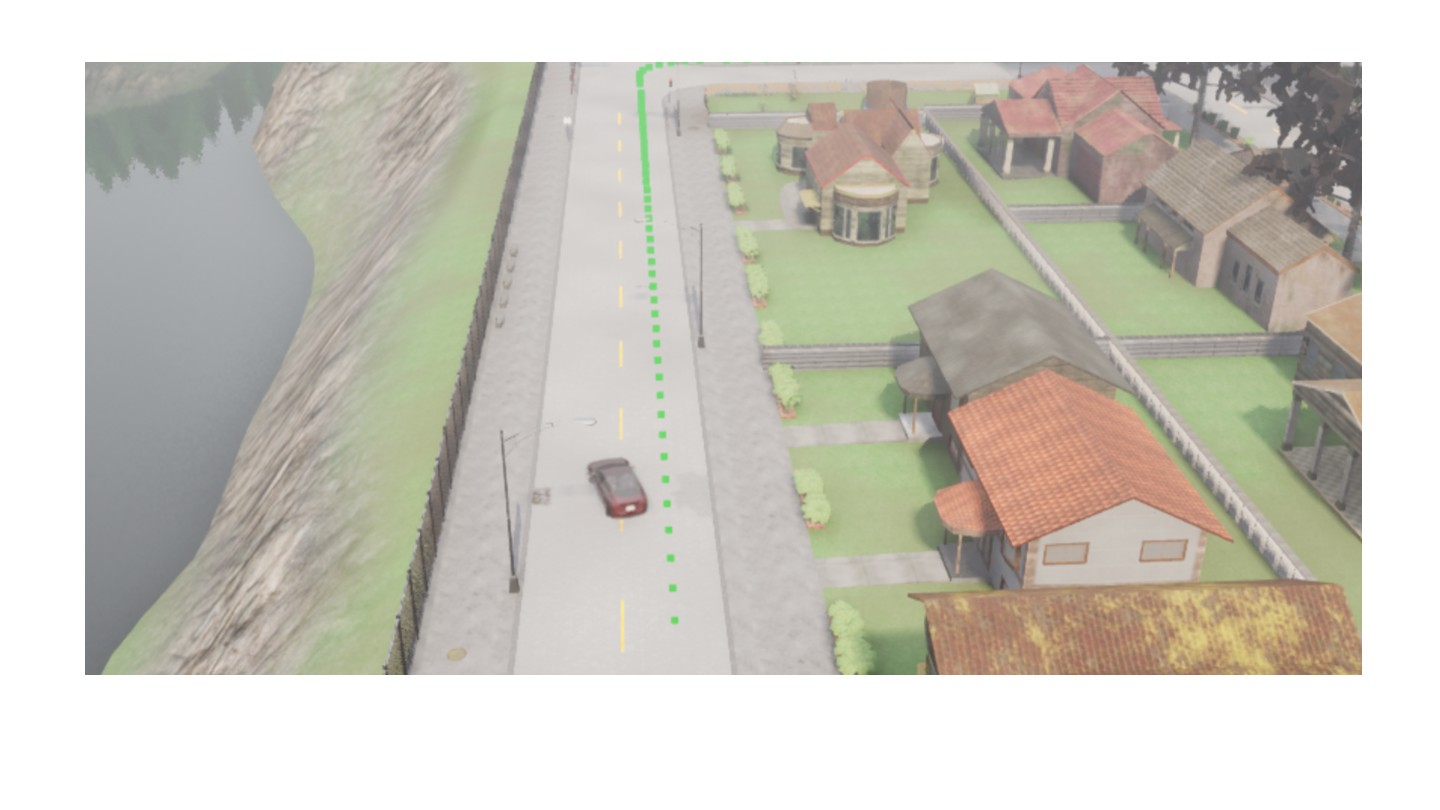
\includegraphics[width=\linewidth]{小车训练图片.jpeg}
	\caption{小车训练图片}
	\label{f.example}
\end{figure}

通过上述方法来进行训练,可以令小车能够按照我们的意愿来进行自动驾驶。我们可以在Carla仿真中的地图上为小车设计小车的起点和终点。使小车能够在我们设计的起点和终点之间进行自动驾驶。


\section{自动驾驶仿真结果分析}


图5-1是测试过程中的典型小车前进的场景,用CARLA旁观者模式的一系列捕捉画面来提供,结果显示在小车前进的过程中,小车通过已经训练好的模型在不偏离我们为小车设定的路径上不断前进。我们可以通过这个测试来查看小车模型的训练情况,从而推测我们所训练的模型是否符合我们的需求。

\begin{figure}[hbt]
	\centering
	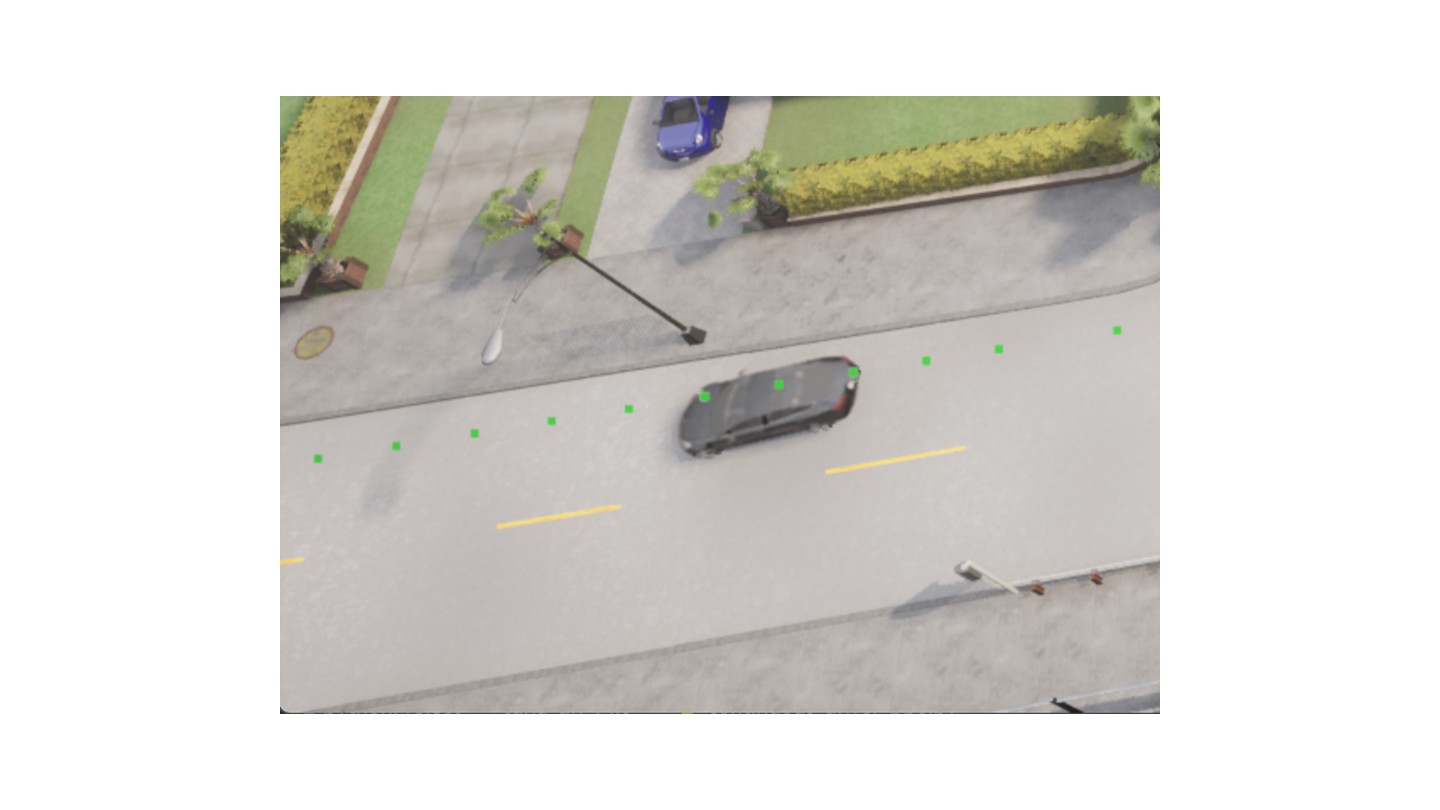
\includegraphics[width=\linewidth]{小车测试图像.jpeg}
	\caption{小车测试图像}
	\label{f.example}
\end{figure}

通过对模型进行训练,我们可以发现,随着训练时间和训练次数的增加。我们训练的模型的效果也会越来越好。我们可以通过如图5-3、5-4的图片对模型的训练效果有一个较为直观的认识。

\begin{figure}[hbt]
	\centering
	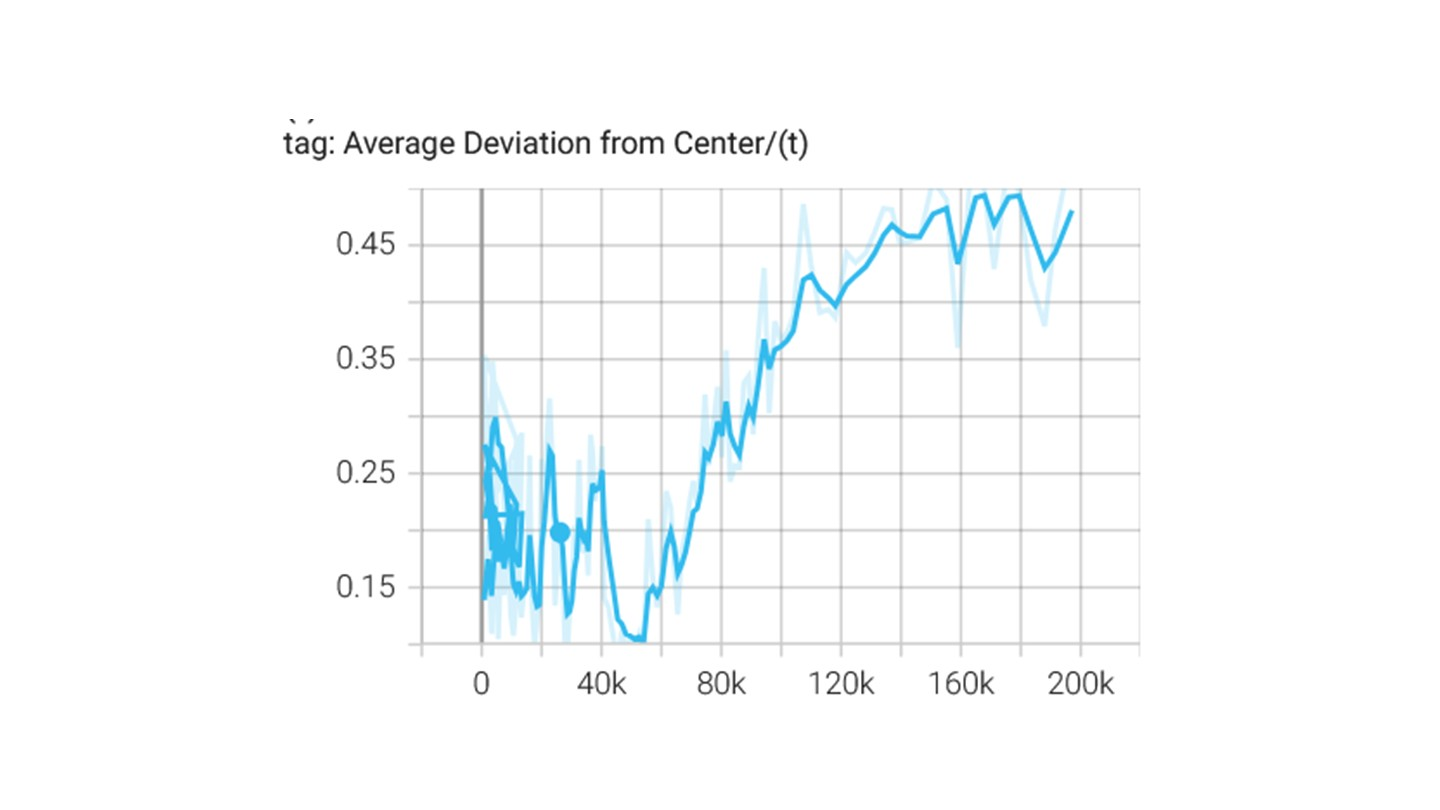
\includegraphics[width=\linewidth]{模型训练图时间.jpeg}
	\caption{模型训练图时间}
	\label{f.example}
\end{figure}


\begin{figure}[hbt]
	\centering
	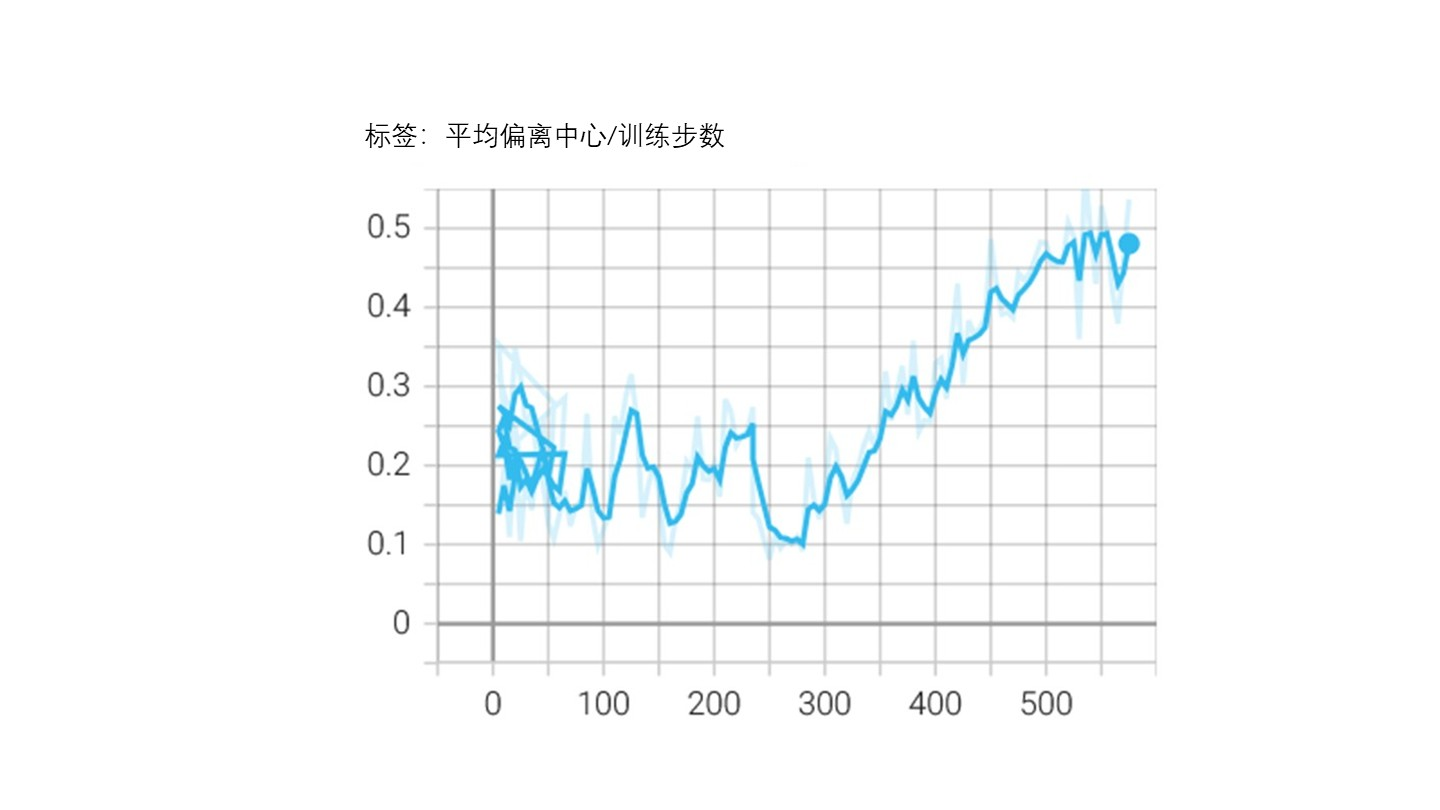
\includegraphics[width=\linewidth]{模型训练图训练次数.jpeg}
	\caption{模型训练图训练次数像}
	\label{f.example}
\end{figure}

通过观察图5-3和图5-4所示的学习过程可视化结果,我们可以清晰的了解机器学习模型在迭代优化过程中的动态演化过程。随着学习周期的不断进行和时间的积累,模型输出与指定的目标路径之间的偏差将表现出更大的收敛趋势。这种量化的改进过程不仅体现在数值分数的降低上,而且通过可视化曲线的形态变化表现出系统性的优化特征。

从训练一开始,参数初始化的随机性往往会导致模型的预测轨迹与理想路径有较大的偏差。此时,损失函数值处于较高范围,表明模型对训练数据的拟合效果仍然不够好。随着梯度下降算法的迭代,模型参数沿着误差曲面梯度的负方向逐渐调整,每次反向传播都使权重矩阵更接近数据特有的规律。这种对参数空间的逐步探索使得模型在面对相同输入值时能够获得接近真实标签的输出,从而有助于形成损失函数值单调递减的优化曲线。


需要注意的是,这个优化过程并非简单的线性递减。在训练中期,当模型初步识别数据分布特征时,损失函数的递减速度会突然加快,在学习曲线上形成“临界点”现象。这标志着模型突破的开始,突破了局部最优的束缚,通过参数空间的调整实现了质的提升。此时,可视化结果中的预测轨迹从离散分布明显转变为收敛到目标路径。这种结构性的提升体现了深度神经网络分层表示学习的优势。

随着训练轮次的推进,模型优化逐渐从全局调整转向微调。此时,损失函数的递减速度有所减缓,但模型输出的稳定性得到了大幅提升,同时对噪声数据的鲁棒性也得到了提升。在可视化结果中,预测路径与目标路径的重叠度越来越大。不仅在训练集上的表现更佳,在验证集上的泛化误差也开始同步下降。这表明模型确实实现了从数据拟合到模式识别的飞跃。

整个学习过程本质上是模型参数与数据特征之间的持续对话。随着迭代次数的增加,神经网络逐层提取特征,将原始数据转化为越来越具有判别力的特征表示。这种提升的表征学习能力使得模型能够以更低的误差成本捕捉数据背后的复杂模式。一旦学习达到收敛,模型不仅在数值层面最小化误差,还在认知层面构建与任务目标高度契合的内部表征体系。这正是深度学习模型在计算机视觉、自然语言处理等领域取得突破的主要机制。








